\documentclass{article}

\usepackage{fancyhdr}
\usepackage{extramarks}
\usepackage{amsmath}
\usepackage{amsthm}
\usepackage{amsfonts}
\usepackage{tikz}
\usepackage[plain]{algorithm}
\usepackage{algpseudocode}
\usepackage{wrapfig}

\usetikzlibrary{automata,positioning}

%
% Basic Document Settings
%

\topmargin=-0.45in
\evensidemargin=0in
\oddsidemargin=0in
\textwidth=6.5in
\textheight=9.0in
\headsep=0.25in

\linespread{1.1}

\pagestyle{fancy}
\lhead{\hmwkAuthorName}
\rhead{\firstxmark}
\lfoot{\lastxmark}
\cfoot{\thepage}

\renewcommand\headrulewidth{0.4pt}
\renewcommand\footrulewidth{0.4pt}

\setlength\parindent{0pt}

%
% Create Problem Sections
%

\newcommand{\enterProblemHeader}[1]{
    \nobreak\extramarks{}{Problem \arabic{#1} continued on next page\ldots}\nobreak{}
    \nobreak\extramarks{Problem \arabic{#1} (continued)}{Problem \arabic{#1} continued on next page\ldots}\nobreak{}
}

\newcommand{\exitProblemHeader}[1]{
    \nobreak\extramarks{Problem \arabic{#1} (continued)}{Problem \arabic{#1} continued on next page\ldots}\nobreak{}
    \stepcounter{#1}
    \nobreak\extramarks{Problem \arabic{#1}}{}\nobreak{}
}

\setcounter{secnumdepth}{0}
\newcounter{partCounter}
\newcounter{homeworkProblemCounter}
\setcounter{homeworkProblemCounter}{1}
\nobreak\extramarks{Problem \arabic{homeworkProblemCounter}}{}\nobreak{}

%
% Homework Problem Environment
%
% This environment takes an optional argument. When given, it will adjust the
% problem counter. This is useful for when the problems given for your
% assignment aren't sequential. See the last 3 problems of this template for an
% example.
%
\newenvironment{homeworkProblem}[1][-1]{
    \ifnum#1>0
        \setcounter{homeworkProblemCounter}{#1}
    \fi
    \section{Problem \arabic{homeworkProblemCounter}}
    \setcounter{partCounter}{1}
    \enterProblemHeader{homeworkProblemCounter}
}{
    \exitProblemHeader{homeworkProblemCounter}
}

%
% Homework Details
%   - Title
%   - Due date
%   - Class
%   - Section/Time
%   - Instructor
%   - Author
%

\newcommand{\hmwkTitle}{Computer Assignment\ \#3}
\newcommand{\hmwkDueDate}{May 12, 2023}
\newcommand{\hmwkClass}{Natural Language Processing}
\newcommand{\hmwkClassTime}{Chapter 9}
\newcommand{\hmwkClassInstructor}{Professor Hesham Faili}
\newcommand{\hmwkAuthorName}{\textbf{Tohid Abdi}}

%
% Title Page
%

\title{
    \vspace{2in}
    \textmd{\textbf{\hmwkClass:\ \hmwkTitle}}\\
    \normalsize\vspace{0.1in}\small{Due\ on\ \hmwkDueDate}\\
    \vspace{3in}
}

\author{\hmwkAuthorName}
\date{}

\renewcommand{\part}[1]{\textbf{\large Part \Alph{partCounter}}\stepcounter{partCounter}\\}

%
% Various Helper Commands
%

% Useful for algorithms
\newcommand{\alg}[1]{\textsc{\bfseries \footnotesize #1}}

% For derivatives
\newcommand{\deriv}[1]{\frac{\mathrm{d}}{\mathrm{d}x} (#1)}

% For partial derivatives
\newcommand{\pderiv}[2]{\frac{\partial}{\partial #1} (#2)}

% Integral dx
\newcommand{\dx}{\mathrm{d}x}

% Alias for the Solution section header
\newcommand{\solution}{\textbf{\large Solution}}

% Probability commands: Expectation, Variance, Covariance, Bias
\newcommand{\E}{\mathrm{E}}
\newcommand{\Var}{\mathrm{Var}}
\newcommand{\Cov}{\mathrm{Cov}}
\newcommand{\Bias}{\mathrm{Bias}}

\begin{document}

\maketitle

\pagebreak

\begin{homeworkProblem}

    \textbf{Preprocessing the Data}

In the first step, we download the data using the download link and extract them. Then we put them in training and testing dataframes.\\

To preprocess the data, we perform the following steps:
\begin{itemize}
  \item Convert all text to lowercase
  \item Expand clitic contractions
  \item Remove URLs
  \item Remove punctuation marks (including hashtags and mentions)
  \item Tokenization
  \item Stop word removal
  \item Stemming
\end{itemize}

We apply these operations on both the training and testing data.\\
    
    \textbf{Training and Evaluating Simple RNN Model}
    
\begin{enumerate}
  \item To perform this task, we used the tokenize function that exists in the nltk library.
  \item We have used One-Hot method and Glove embeddings to convert the words into suitable vectors.
  \item We have used the pad\_sequence function for this task. Applying padding on the right side of the sentences causes loss of information and weakens the performance of the model. Therefore, we apply padding on the right side of the sentencs.
  \item To apply RNN in this setting, we pass the text to be classified through the RNN a word at a time generating a new hidden layer at each time step. We can then take the hidden layer for the last token of the text, $h_{n}$, to constitute a compressed representation of the entire sequence. We can pass this representation $h_{n}$ to a feedforward network that chooses a class via a softmax over the possible classes.  Fig. 1 illustrates this approach.
      
\begin{figure}[h]
    \centering
    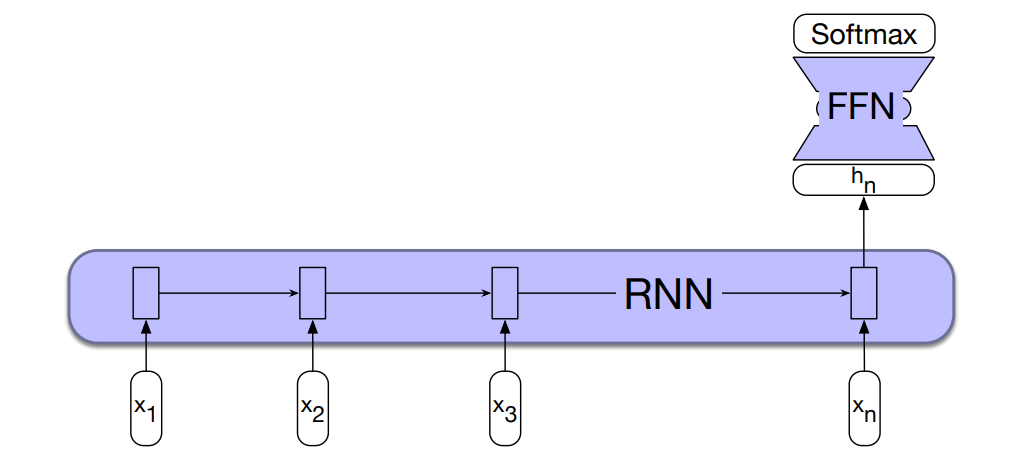
\includegraphics{model.png}
    \caption{Sequence classification using a simple RNN combined with a feedforward network}
    \end{figure}
      
  \item Done!
  \item Due to the fact that the training data had two classes, positive and negative, and there was no neutral class in them, we removed data with a neutral class from the test data. The confusion matrix for the test data is as follows:
      
\begin{table}[h]
    \centering
    \caption{Confusion Matrix for test data using one-hot Embedding\\}   \begin{tabular}{|c|cc|}
        \hline
        - & Actual 0 & Actual 1  \\ \hline
        0 Predicted & 102 & 107\\
        1 Predicted & 75 & 75\\ \hline
    \end{tabular}
\end{table}

\begin{table}[h]
    \centering
    \caption{Confusion Matrix for test data using Glove Embedding\\}   \begin{tabular}{|c|cc|}
        \hline
        - & Actual 0 & Actual 1  \\ \hline
        0 Predicted & 134 & 42\\
        1 Predicted & 43 & 140\\ \hline
    \end{tabular}
\end{table}


\end{enumerate}





\end{homeworkProblem}

\pagebreak



\begin{homeworkProblem}

    \textbf{Training and Evaluating LSTM and GRU Models}
    
\begin{enumerate}
  \item We use nn.LSTM layer to implement LSTM layer
  \item Done!
  \item We set the criterion equal to the nn.CrossEntropyLoss()
  \item We have used the one-hot method and Glove embedding. Like RNN, using Glove embedding improved the performance of the model.
  \item The confusion matrix for the test data is as follows:
      
\begin{table}[h]
    \centering
    \caption{Confusion Matrix for LSTM Model using one-hot Embedding\\}   \begin{tabular}{|c|cc|}
        \hline
        - & Actual 0 & Actual 1  \\ \hline
        0 Predicted & 103 & 106\\
        1 Predicted & 74 & 76\\ \hline
    \end{tabular}
\end{table}

\begin{table}[h]
    \centering
    \caption{Confusion Matrix for LSTM Model using Glove Embedding\\}   \begin{tabular}{|c|cc|}
        \hline
        - & Actual 0 & Actual 1  \\ \hline
        0 Predicted & 138 & 42\\
        1 Predicted & 39 & 140\\ \hline
    \end{tabular}
\end{table}

When we use the one-hot method, our model has a performance almost close to random selection, but using Glove embedding increases the accuracy of the model in separating classes.

  \item We use nn.GRU layer to implement GRU layer
  \item The confusion matrix for the test data is as follows:
      
\begin{table}[h]
    \centering
    \caption{Confusion Matrix for GRU Model using one-hot Embedding\\}   \begin{tabular}{|c|cc|}
        \hline
        - & Actual 0 & Actual 1  \\ \hline
        0 Predicted & 103 & 119\\
        1 Predicted & 74 & 63\\ \hline
    \end{tabular}
\end{table}

\pagebreak

\begin{table}[h]
    \centering
    \caption{Confusion Matrix for GRU Model using Glove Embedding\\}   \begin{tabular}{|c|cc|}
        \hline
        - & Actual 0 & Actual 1  \\ \hline
        0 Predicted & 132 & 41\\
        1 Predicted & 45 & 141\\ \hline
    \end{tabular}
\end{table}

Each epoch in LSTM model with Glove embedding takes 9 seconds, but while using GRU it only takes roughly 15 seconds.\\

Table 7 shows the general performance of different models.

\begin{table}[h]
    \centering
    \caption{Accuracy of prediction with different models\\}   \begin{tabular}{|c|c|c|}
        \hline
        - & One-Hot embedding & GloVe  \\ \hline
        Simple RNN & 0.493 & 0.7632\\
        LSTM & 0.4986 & 0.7744\\
        RNN & 0.4624 & 0.7604\\ \hline
    \end{tabular}
\end{table}

\end{enumerate}


\end{homeworkProblem}

\end{document}
